\PassOptionsToPackage{unicode=true}{hyperref} % options for packages loaded elsewhere
\PassOptionsToPackage{hyphens}{url}
%
\documentclass[]{article}
\usepackage{lmodern}
\usepackage{amssymb,amsmath}
\usepackage{ifxetex,ifluatex}
\usepackage{fixltx2e} % provides \textsubscript
\ifnum 0\ifxetex 1\fi\ifluatex 1\fi=0 % if pdftex
  \usepackage[T1]{fontenc}
  \usepackage[utf8]{inputenc}
  \usepackage{textcomp} % provides euro and other symbols
\else % if luatex or xelatex
  \usepackage{unicode-math}
  \defaultfontfeatures{Ligatures=TeX,Scale=MatchLowercase}
\fi
% use upquote if available, for straight quotes in verbatim environments
\IfFileExists{upquote.sty}{\usepackage{upquote}}{}
% use microtype if available
\IfFileExists{microtype.sty}{%
\usepackage[]{microtype}
\UseMicrotypeSet[protrusion]{basicmath} % disable protrusion for tt fonts
}{}
\IfFileExists{parskip.sty}{%
\usepackage{parskip}
}{% else
\setlength{\parindent}{0pt}
\setlength{\parskip}{6pt plus 2pt minus 1pt}
}
\usepackage{hyperref}
\hypersetup{
            pdftitle={Testing sbmlogit package},
            pdfauthor={Carter Allen},
            pdfborder={0 0 0},
            breaklinks=true}
\urlstyle{same}  % don't use monospace font for urls
\usepackage[margin=1in]{geometry}
\usepackage{color}
\usepackage{fancyvrb}
\newcommand{\VerbBar}{|}
\newcommand{\VERB}{\Verb[commandchars=\\\{\}]}
\DefineVerbatimEnvironment{Highlighting}{Verbatim}{commandchars=\\\{\}}
% Add ',fontsize=\small' for more characters per line
\usepackage{framed}
\definecolor{shadecolor}{RGB}{248,248,248}
\newenvironment{Shaded}{\begin{snugshade}}{\end{snugshade}}
\newcommand{\AlertTok}[1]{\textcolor[rgb]{0.94,0.16,0.16}{#1}}
\newcommand{\AnnotationTok}[1]{\textcolor[rgb]{0.56,0.35,0.01}{\textbf{\textit{#1}}}}
\newcommand{\AttributeTok}[1]{\textcolor[rgb]{0.77,0.63,0.00}{#1}}
\newcommand{\BaseNTok}[1]{\textcolor[rgb]{0.00,0.00,0.81}{#1}}
\newcommand{\BuiltInTok}[1]{#1}
\newcommand{\CharTok}[1]{\textcolor[rgb]{0.31,0.60,0.02}{#1}}
\newcommand{\CommentTok}[1]{\textcolor[rgb]{0.56,0.35,0.01}{\textit{#1}}}
\newcommand{\CommentVarTok}[1]{\textcolor[rgb]{0.56,0.35,0.01}{\textbf{\textit{#1}}}}
\newcommand{\ConstantTok}[1]{\textcolor[rgb]{0.00,0.00,0.00}{#1}}
\newcommand{\ControlFlowTok}[1]{\textcolor[rgb]{0.13,0.29,0.53}{\textbf{#1}}}
\newcommand{\DataTypeTok}[1]{\textcolor[rgb]{0.13,0.29,0.53}{#1}}
\newcommand{\DecValTok}[1]{\textcolor[rgb]{0.00,0.00,0.81}{#1}}
\newcommand{\DocumentationTok}[1]{\textcolor[rgb]{0.56,0.35,0.01}{\textbf{\textit{#1}}}}
\newcommand{\ErrorTok}[1]{\textcolor[rgb]{0.64,0.00,0.00}{\textbf{#1}}}
\newcommand{\ExtensionTok}[1]{#1}
\newcommand{\FloatTok}[1]{\textcolor[rgb]{0.00,0.00,0.81}{#1}}
\newcommand{\FunctionTok}[1]{\textcolor[rgb]{0.00,0.00,0.00}{#1}}
\newcommand{\ImportTok}[1]{#1}
\newcommand{\InformationTok}[1]{\textcolor[rgb]{0.56,0.35,0.01}{\textbf{\textit{#1}}}}
\newcommand{\KeywordTok}[1]{\textcolor[rgb]{0.13,0.29,0.53}{\textbf{#1}}}
\newcommand{\NormalTok}[1]{#1}
\newcommand{\OperatorTok}[1]{\textcolor[rgb]{0.81,0.36,0.00}{\textbf{#1}}}
\newcommand{\OtherTok}[1]{\textcolor[rgb]{0.56,0.35,0.01}{#1}}
\newcommand{\PreprocessorTok}[1]{\textcolor[rgb]{0.56,0.35,0.01}{\textit{#1}}}
\newcommand{\RegionMarkerTok}[1]{#1}
\newcommand{\SpecialCharTok}[1]{\textcolor[rgb]{0.00,0.00,0.00}{#1}}
\newcommand{\SpecialStringTok}[1]{\textcolor[rgb]{0.31,0.60,0.02}{#1}}
\newcommand{\StringTok}[1]{\textcolor[rgb]{0.31,0.60,0.02}{#1}}
\newcommand{\VariableTok}[1]{\textcolor[rgb]{0.00,0.00,0.00}{#1}}
\newcommand{\VerbatimStringTok}[1]{\textcolor[rgb]{0.31,0.60,0.02}{#1}}
\newcommand{\WarningTok}[1]{\textcolor[rgb]{0.56,0.35,0.01}{\textbf{\textit{#1}}}}
\usepackage{graphicx,grffile}
\makeatletter
\def\maxwidth{\ifdim\Gin@nat@width>\linewidth\linewidth\else\Gin@nat@width\fi}
\def\maxheight{\ifdim\Gin@nat@height>\textheight\textheight\else\Gin@nat@height\fi}
\makeatother
% Scale images if necessary, so that they will not overflow the page
% margins by default, and it is still possible to overwrite the defaults
% using explicit options in \includegraphics[width, height, ...]{}
\setkeys{Gin}{width=\maxwidth,height=\maxheight,keepaspectratio}
\setlength{\emergencystretch}{3em}  % prevent overfull lines
\providecommand{\tightlist}{%
  \setlength{\itemsep}{0pt}\setlength{\parskip}{0pt}}
\setcounter{secnumdepth}{0}
% Redefines (sub)paragraphs to behave more like sections
\ifx\paragraph\undefined\else
\let\oldparagraph\paragraph
\renewcommand{\paragraph}[1]{\oldparagraph{#1}\mbox{}}
\fi
\ifx\subparagraph\undefined\else
\let\oldsubparagraph\subparagraph
\renewcommand{\subparagraph}[1]{\oldsubparagraph{#1}\mbox{}}
\fi

% set default figure placement to htbp
\makeatletter
\def\fps@figure{htbp}
\makeatother


\title{Testing sbmlogit package}
\author{Carter Allen}
\date{1/20/2020}

\begin{document}
\maketitle

{
\setcounter{tocdepth}{2}
\tableofcontents
}
\hypertarget{to-do}{%
\section{To-Do}\label{to-do}}

\begin{itemize}
\tightlist
\item
  Create plotting functions
\item
  Assess the effect of degree correction (see P \& C section 7.2.1)
\item
  Fit models to more test data sets of differing community structure
\item
  Look into model comparison criteria
\item
  Look into model extensions
\item
  Better understand interpretation of model parameters
\end{itemize}

\hypertarget{intro}{%
\section{Intro}\label{intro}}

Load packages. \texttt{igraph} is required, as well as the \texttt{C}
library version.

\begin{Shaded}
\begin{Highlighting}[]
\KeywordTok{library}\NormalTok{(igraph)}
\KeywordTok{library}\NormalTok{(igraphdata)}
\KeywordTok{library}\NormalTok{(sbmlogit)}
\KeywordTok{library}\NormalTok{(sbmlhelpers)}
\KeywordTok{library}\NormalTok{(ggraph)}
\KeywordTok{library}\NormalTok{(tidygraph)}
\KeywordTok{library}\NormalTok{(tidyverse)}
\KeywordTok{library}\NormalTok{(coda)}
\end{Highlighting}
\end{Shaded}

\hypertarget{karate-data}{%
\section{Karate Data}\label{karate-data}}

Load karate data (an \texttt{igraph} object). Note that
\texttt{sbmlogit} operates on data in the form of \texttt{igraph}
objects.

\begin{Shaded}
\begin{Highlighting}[]
\KeywordTok{data}\NormalTok{(}\StringTok{"karate"}\NormalTok{)}
\end{Highlighting}
\end{Shaded}

Obtain MCMC samples for \(K = 2\) specified clusters. We can specify a
two cluster model by setting \texttt{alpha\ =\ 2}, in which case \(K\)
is set automatically to 2, and \(\alpha\) is set to
\(\alpha_{K \times 1} = (1/K,...,1/K)^T\). The number of MCMC iterations
is controlled with \texttt{nsamples}.

\begin{Shaded}
\begin{Highlighting}[]
\NormalTok{fitK2 <-}\StringTok{ }\KeywordTok{sbmlogit.mcmc}\NormalTok{(}\DataTypeTok{graph =}\NormalTok{ karate,}\DataTypeTok{alpha =} \DecValTok{2}\NormalTok{,}\DataTypeTok{nsamples =} \DecValTok{2000}\NormalTok{)}
\end{Highlighting}
\end{Shaded}

Define the \texttt{mp} (``most probable''?) function from P \& C (2016),
where \texttt{apply(Sigma,\ 2,\ mp,\ K)} returns a \(K \times N\)
matrix, the transpose of which is the \({N \times K}\) matrix
\(\mathbf{P}\), where \(P_{ij}\) is the proportion of MCMC iterations
where node \(i\) (\(i = 1,...,N\)) belonged to cluster \(j\)
(\(j = 1,...,K\)).

\begin{Shaded}
\begin{Highlighting}[]
\CommentTok{# Function for estimator}
\NormalTok{mp =}\StringTok{ }\ControlFlowTok{function}\NormalTok{(vec, K)\{}
\NormalTok{  v =}\StringTok{ }\KeywordTok{rep}\NormalTok{(}\DecValTok{1}\OperatorTok{:}\NormalTok{K)}
\NormalTok{  l =}\StringTok{ }\KeywordTok{length}\NormalTok{(vec)}
  
  \ControlFlowTok{for}\NormalTok{ (i }\ControlFlowTok{in} \DecValTok{1}\OperatorTok{:}\NormalTok{K)\{}
\NormalTok{    v[i] =}\StringTok{ }\KeywordTok{sum}\NormalTok{(vec}\OperatorTok{==}\NormalTok{i)}\OperatorTok{/}\NormalTok{l}
\NormalTok{  \}}
  \KeywordTok{return}\NormalTok{(v)}
\NormalTok{\}}
\end{Highlighting}
\end{Shaded}

Now, we apply the \texttt{which.max()} function to the matrix
\(\mathbf{P}\) described above to find the most probable cluster
membership for each node. The \texttt{sbmlogit.remap()} function remaps
the posterior estimate of \(\boldsymbol\sigma\) to the canonical version
described in P \& C (2016).

Compute estimators.

\begin{Shaded}
\begin{Highlighting}[]
\NormalTok{SigmaK2 <-}\StringTok{ }\NormalTok{fitK2}\OperatorTok{$}\NormalTok{sample }\CommentTok{# posterior samples}
\NormalTok{sigmaK2 <-}\StringTok{ }\KeywordTok{apply}\NormalTok{(}\KeywordTok{t}\NormalTok{(}\KeywordTok{apply}\NormalTok{(SigmaK2, }\DecValTok{2}\NormalTok{, mp, }\DecValTok{2}\NormalTok{)), }\DecValTok{1}\NormalTok{, which.max) }\CommentTok{# posterior estimator}
\NormalTok{scentroidK2 <-}\StringTok{ }\KeywordTok{sbmlogit.remap}\NormalTok{(sigmaK2) }\CommentTok{# remapped posterior estimator}
\KeywordTok{print}\NormalTok{(scentroidK2)}
\end{Highlighting}
\end{Shaded}

\begin{verbatim}
##  [1] 1 1 1 1 1 1 1 1 2 2 1 1 1 1 2 2 1 1 2 1 2 1 2 2 2 2 2 2 2 2 2 2 2 2
\end{verbatim}

Evaluate model fit with WAIC.

\begin{Shaded}
\begin{Highlighting}[]
\CommentTok{# function to compute WAIC}
\CommentTok{# verify this is correct}
\NormalTok{waic <-}\StringTok{ }\ControlFlowTok{function}\NormalTok{(fit,}\DataTypeTok{burn =} \DecValTok{0}\NormalTok{)}
\NormalTok{\{}
\NormalTok{    S <-}\StringTok{ }\KeywordTok{length}\NormalTok{(fit}\OperatorTok{$}\NormalTok{lhood)}
\NormalTok{    ls <-}\StringTok{ }\KeywordTok{exp}\NormalTok{(fit}\OperatorTok{$}\NormalTok{lhood[(burn}\OperatorTok{+}\DecValTok{1}\NormalTok{)}\OperatorTok{:}\NormalTok{S])}
\NormalTok{    w <-}\StringTok{ }\DecValTok{2}\OperatorTok{*}\NormalTok{(}\KeywordTok{log}\NormalTok{(}\KeywordTok{mean}\NormalTok{(ls)) }\OperatorTok{-}\StringTok{ }\KeywordTok{mean}\NormalTok{(}\KeywordTok{log}\NormalTok{(ls)))}
    \KeywordTok{return}\NormalTok{(w)}
\NormalTok{\}}
\end{Highlighting}
\end{Shaded}

Compare models with varying K.

\begin{Shaded}
\begin{Highlighting}[]
\NormalTok{fitK3 <-}\StringTok{ }\KeywordTok{sbmlogit.mcmc}\NormalTok{(}\DataTypeTok{graph =}\NormalTok{ karate,}\DataTypeTok{alpha =} \DecValTok{3}\NormalTok{,}\DataTypeTok{nsamples =} \DecValTok{1000}\NormalTok{)}
\NormalTok{fitK4 <-}\StringTok{ }\KeywordTok{sbmlogit.mcmc}\NormalTok{(}\DataTypeTok{graph =}\NormalTok{ karate,}\DataTypeTok{alpha =} \DecValTok{4}\NormalTok{,}\DataTypeTok{nsamples =} \DecValTok{1000}\NormalTok{)}
\NormalTok{fitK5 <-}\StringTok{ }\KeywordTok{sbmlogit.mcmc}\NormalTok{(}\DataTypeTok{graph =}\NormalTok{ karate,}\DataTypeTok{alpha =} \DecValTok{5}\NormalTok{,}\DataTypeTok{nsamples =} \DecValTok{1000}\NormalTok{)}
\end{Highlighting}
\end{Shaded}

\begin{Shaded}
\begin{Highlighting}[]
\KeywordTok{waic}\NormalTok{(fitK2, }\DataTypeTok{burn =} \DecValTok{100}\NormalTok{)}
\end{Highlighting}
\end{Shaded}

\begin{verbatim}
## [1] 36.11339
\end{verbatim}

\begin{Shaded}
\begin{Highlighting}[]
\KeywordTok{waic}\NormalTok{(fitK3, }\DataTypeTok{burn =} \DecValTok{100}\NormalTok{)}
\end{Highlighting}
\end{Shaded}

\begin{verbatim}
## [1] 53.68402
\end{verbatim}

\begin{Shaded}
\begin{Highlighting}[]
\KeywordTok{waic}\NormalTok{(fitK4, }\DataTypeTok{burn =} \DecValTok{100}\NormalTok{)}
\end{Highlighting}
\end{Shaded}

\begin{verbatim}
## [1] Inf
\end{verbatim}

\begin{Shaded}
\begin{Highlighting}[]
\KeywordTok{waic}\NormalTok{(fitK5, }\DataTypeTok{burn =} \DecValTok{100}\NormalTok{)}
\end{Highlighting}
\end{Shaded}

\begin{verbatim}
## [1] Inf
\end{verbatim}

Alternatively, we could inventigate posterior distributions of model
log-likelihood. We note however that this approach does not properly
penalize for model complexity.

\begin{Shaded}
\begin{Highlighting}[]
\NormalTok{lls_df <-}\StringTok{ }\KeywordTok{as.data.frame}\NormalTok{(}\KeywordTok{cbind}\NormalTok{(fitK2}\OperatorTok{$}\NormalTok{lhood,fitK3}\OperatorTok{$}\NormalTok{lhood,fitK4}\OperatorTok{$}\NormalTok{lhood,fitK5}\OperatorTok{$}\NormalTok{lhood))}
\KeywordTok{colnames}\NormalTok{(lls_df) <-}\StringTok{ }\KeywordTok{c}\NormalTok{(}\StringTok{"K2"}\NormalTok{,}\StringTok{"K3"}\NormalTok{,}\StringTok{"K4"}\NormalTok{,}\StringTok{"K5"}\NormalTok{)}
\NormalTok{lls_df <-}\StringTok{ }\NormalTok{lls_df }\OperatorTok\StringTok{ }
\StringTok{  }\KeywordTok{gather}\NormalTok{(}\DataTypeTok{key =} \StringTok{"Model"}\NormalTok{, }\DataTypeTok{value =} \StringTok{"ll"}\NormalTok{)}
\KeywordTok{ggplot}\NormalTok{(}\DataTypeTok{data =}\NormalTok{ lls_df,}
       \KeywordTok{aes}\NormalTok{(}\DataTypeTok{x =}\NormalTok{ ll)) }\OperatorTok{+}\StringTok{ }
\StringTok{  }\KeywordTok{geom_histogram}\NormalTok{(}\DataTypeTok{bins =} \DecValTok{30}\NormalTok{) }\OperatorTok{+}\StringTok{ }
\StringTok{  }\KeywordTok{facet_wrap}\NormalTok{(}\OperatorTok{~}\StringTok{ }\NormalTok{Model, }\DataTypeTok{nrow =} \DecValTok{4}\NormalTok{) }\OperatorTok{+}
\StringTok{  }\KeywordTok{scale_x_continuous}\NormalTok{(}\DataTypeTok{limits =} \KeywordTok{c}\NormalTok{(}\OperatorTok{-}\DecValTok{500}\NormalTok{,}\OperatorTok{-}\DecValTok{200}\NormalTok{))}
\end{Highlighting}
\end{Shaded}

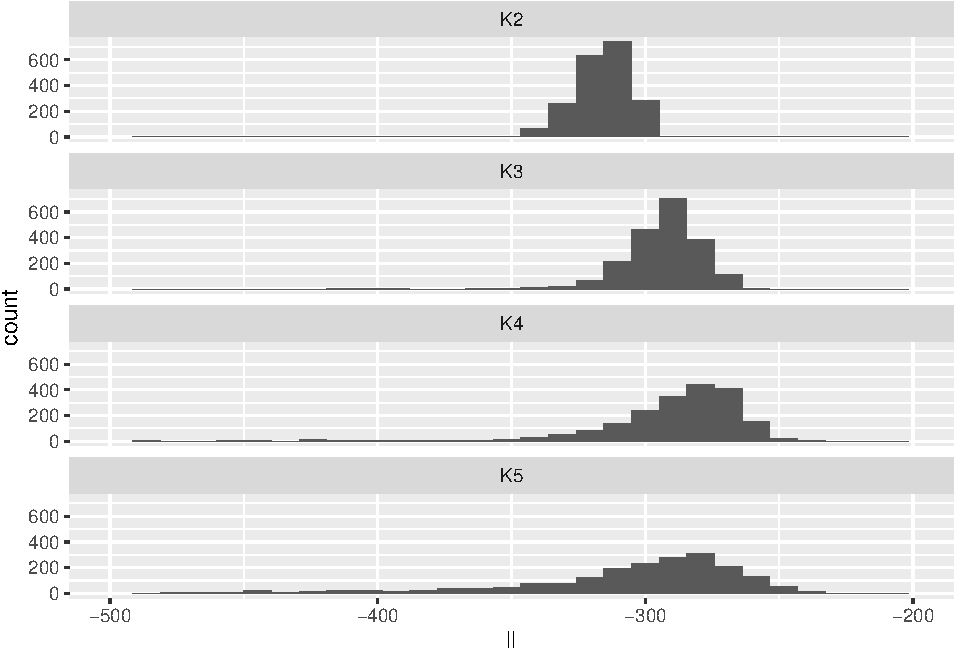
\includegraphics{karate_test_files/figure-latex/unnamed-chunk-9-1.pdf}

Next, let's conduct posterior inference for 2-class model. In this case,
\texttt{fitK2\$gamma} contains the posterior samples of \(\gamma_{12}\).
In general, there are \(K \choose 2\) of the \(\gamma\) parameters:
\(\gamma_{12},...,\gamma_{K-1,K}\), since the authors set
\(\gamma_{11} = \gamma_{22} = ... = \gamma_{KK} = 0\) for
identifiability purposes. Below is a summary of the posterior
distribution of \(\gamma_{12}\) for the two cluster model.

\begin{Shaded}
\begin{Highlighting}[]
\KeywordTok{mean_CRI}\NormalTok{(fitK2}\OperatorTok{$}\NormalTok{gamma)}
\end{Highlighting}
\end{Shaded}

\begin{verbatim}
## [1] "-3.96 (-5.5, -2.86)"
\end{verbatim}

We can see that the posterior mean and 95\% credible interval for
\(\gamma_{12}\) are less than 0 -- the intra-community connectivity of
the graph enforced by assuming \(\gamma_{11} = \gamma_{22} = 0\). Thus,
there is significantly less propensity for edges to exist \emph{between}
the two communities than \emph{within} the two communities. This is
indicative of strong assortative community structure.

The remaining parameters to infer are \(\eta_1,...,\eta_{N}\), where
\(N = 34\) is the number of nodes in the karate graph. Each \(\eta_i\)
accounts for the expected degree of node \(i\) on the logit scale. The
authors refer to this as \emph{node correction} as well as the more
common \emph{degree correction}. Thus, \(\text{logit}^{-1}(\eta_i)\) is
the expected degree of node \(i\).

\begin{Shaded}
\begin{Highlighting}[]
\NormalTok{expit <-}\StringTok{ }\ControlFlowTok{function}\NormalTok{(l)}
\NormalTok{\{}
  \KeywordTok{return}\NormalTok{(}\KeywordTok{exp}\NormalTok{(l)}\OperatorTok{/}\NormalTok{(}\DecValTok{1}\OperatorTok{+}\KeywordTok{exp}\NormalTok{(l)))}
\NormalTok{\}}
\end{Highlighting}
\end{Shaded}

\begin{Shaded}
\begin{Highlighting}[]
\KeywordTok{expit}\NormalTok{(}\KeywordTok{colMeans}\NormalTok{(fitK2}\OperatorTok{$}\NormalTok{eta))}
\end{Highlighting}
\end{Shaded}

\begin{verbatim}
##  [1] 0.95515258 0.76416645 0.80089788 0.52329408 0.17773659 0.29809708
##  [7] 0.29316696 0.29922520 0.40022617 0.09063045 0.17792511 0.03200290
## [13] 0.08929766 0.40905509 0.09689979 0.09966598 0.09793005 0.09469525
## [19] 0.08782846 0.17894335 0.09569812 0.09139508 0.08978369 0.41489586
## [25] 0.17370586 0.18968473 0.09638840 0.28989038 0.18866684 0.29587626
## [31] 0.29344243 0.51625086 0.85896004 0.95431478
\end{verbatim}

We can see that the nodes with the highest expected degree are the
actual ``hubs'' (i.e., the karate teachers), as the \texttt{karate} data
are arranged such that the first and the last nodes are the two karate
teachers.

To plot the estimated communities of the graph, we can use the custom
function \texttt{plot\_sbmlogit()}.

\begin{Shaded}
\begin{Highlighting}[]
\KeywordTok{plot_sbmlogit}\NormalTok{(fitK2, }\DataTypeTok{ground =} \StringTok{"color"}\NormalTok{)}
\end{Highlighting}
\end{Shaded}

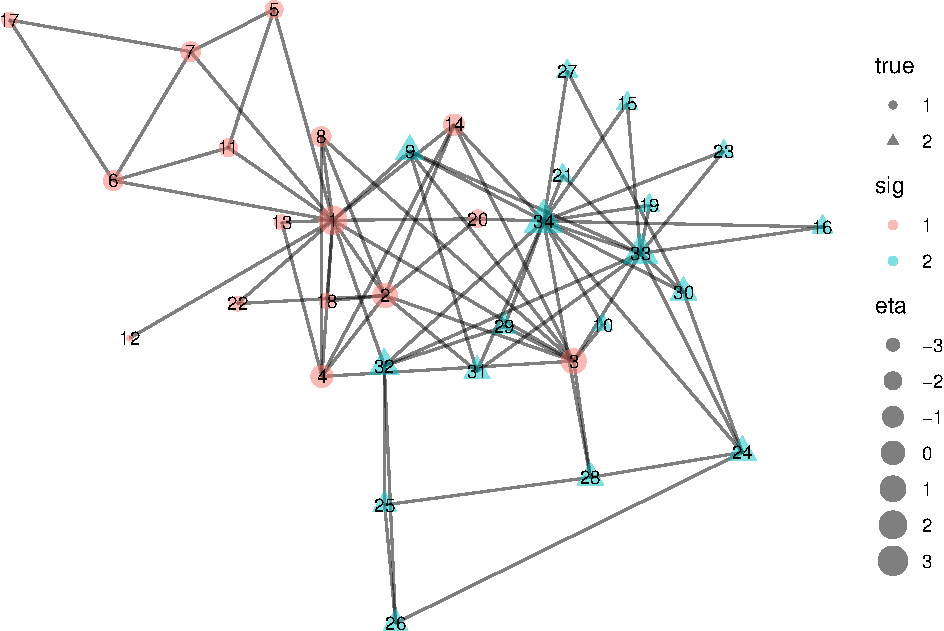
\includegraphics{karate_test_files/figure-latex/unnamed-chunk-13-1.pdf}

\hypertarget{uk-faculty-network}{%
\section{UK Faculty Network}\label{uk-faculty-network}}

The UK faculty network data set is an \texttt{igraph} data set included
in the \texttt{igraphdata} package. The network consists of friendships
between 81 faculty at a university in the UK, with 817 directed and
weighted edges. First, let's read in the \texttt{UKfaculty} data and
save it as an undirected version, \texttt{UKfac}.

\begin{Shaded}
\begin{Highlighting}[]
\KeywordTok{data}\NormalTok{(}\StringTok{"UKfaculty"}\NormalTok{)}
\NormalTok{UKfac <-}\StringTok{ }\KeywordTok{as.undirected}\NormalTok{(UKfaculty)}
\end{Highlighting}
\end{Shaded}

In the \texttt{UKfac} data, each individual's school is saved to the
\texttt{Group} node attribute. We can use this information to obtain a
view of the possible ground truth community memberships.

\begin{Shaded}
\begin{Highlighting}[]
\NormalTok{UKfac <-}\StringTok{ }\NormalTok{UKfac }\OperatorTok
\StringTok{  }\KeywordTok{as_tbl_graph}\NormalTok{() }\OperatorTok
\StringTok{  }\KeywordTok{activate}\NormalTok{(nodes) }\OperatorTok
\StringTok{  }\KeywordTok{mutate}\NormalTok{(}\DataTypeTok{school =} \KeywordTok{as.factor}\NormalTok{(Group)) }\OperatorTok
\StringTok{  }\KeywordTok{as.igraph}\NormalTok{()}
\end{Highlighting}
\end{Shaded}

\begin{Shaded}
\begin{Highlighting}[]
\KeywordTok{ggraph}\NormalTok{(UKfac,}\DataTypeTok{layout =} \StringTok{"kk"}\NormalTok{) }\OperatorTok{+}
\StringTok{  }\KeywordTok{geom_edge_link}\NormalTok{(}\DataTypeTok{alpha =} \FloatTok{0.25}\NormalTok{) }\OperatorTok{+}\StringTok{ }
\StringTok{  }\KeywordTok{geom_node_point}\NormalTok{(}\DataTypeTok{size =} \DecValTok{4}\NormalTok{, }\KeywordTok{aes}\NormalTok{(}\DataTypeTok{color =}\NormalTok{ school)) }\OperatorTok{+}\StringTok{ }
\StringTok{  }\KeywordTok{theme_void}\NormalTok{()}
\end{Highlighting}
\end{Shaded}

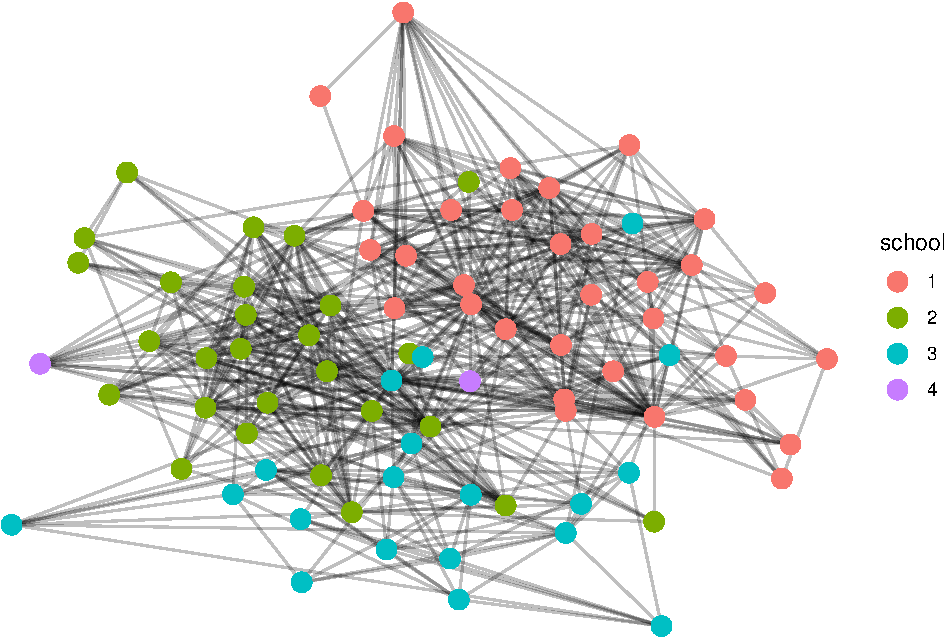
\includegraphics{karate_test_files/figure-latex/unnamed-chunk-16-1.pdf}

As before, we can fit SBM logit models with varying values of K and
assess model fit using WAIC.

\begin{Shaded}
\begin{Highlighting}[]
\NormalTok{fitK2 <-}\StringTok{ }\KeywordTok{sbmlogit.mcmc}\NormalTok{(UKfac,}\DataTypeTok{alpha =} \DecValTok{2}\NormalTok{,}\DataTypeTok{nsamples =} \DecValTok{5000}\NormalTok{)}
\NormalTok{fitK3 <-}\StringTok{ }\KeywordTok{sbmlogit.mcmc}\NormalTok{(UKfac,}\DataTypeTok{alpha =} \DecValTok{3}\NormalTok{,}\DataTypeTok{nsamples =} \DecValTok{5000}\NormalTok{)}
\NormalTok{fitK4 <-}\StringTok{ }\KeywordTok{sbmlogit.mcmc}\NormalTok{(UKfac,}\DataTypeTok{alpha =} \DecValTok{4}\NormalTok{,}\DataTypeTok{nsamples =} \DecValTok{5000}\NormalTok{)}
\NormalTok{fitK5 <-}\StringTok{ }\KeywordTok{sbmlogit.mcmc}\NormalTok{(UKfac,}\DataTypeTok{alpha =} \DecValTok{5}\NormalTok{,}\DataTypeTok{nsamples =} \DecValTok{5000}\NormalTok{)}
\end{Highlighting}
\end{Shaded}

\begin{Shaded}
\begin{Highlighting}[]
\KeywordTok{plot_sbmlogit}\NormalTok{(fitK2,}\DataTypeTok{ground =} \StringTok{"school"}\NormalTok{,}\DataTypeTok{alpha =} \FloatTok{0.25}\NormalTok{)}
\end{Highlighting}
\end{Shaded}

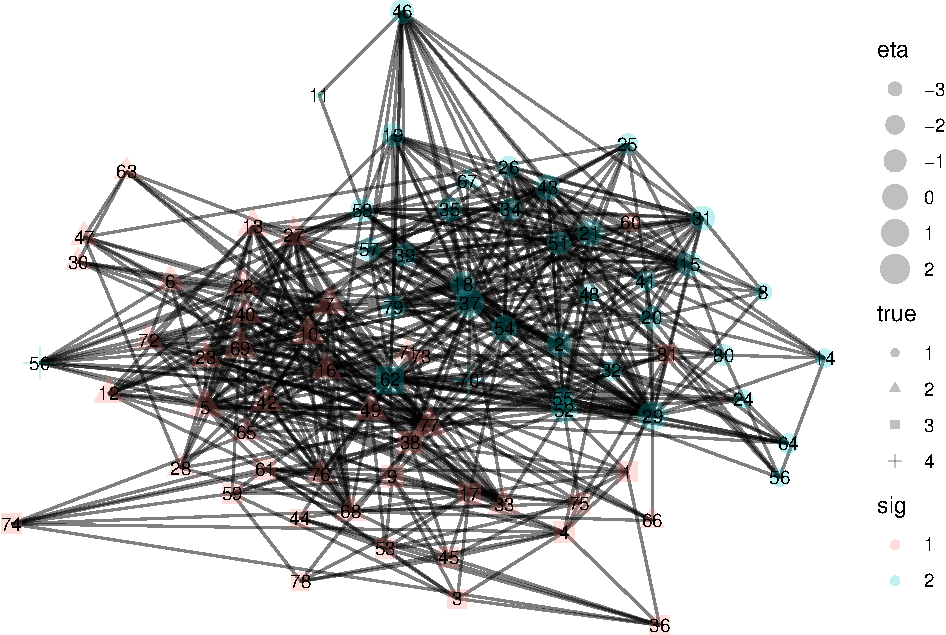
\includegraphics{karate_test_files/figure-latex/unnamed-chunk-18-1.pdf}

\begin{Shaded}
\begin{Highlighting}[]
\KeywordTok{plot_sbmlogit}\NormalTok{(fitK3,}\DataTypeTok{ground =} \StringTok{"school"}\NormalTok{, }\DataTypeTok{alpha =} \FloatTok{0.25}\NormalTok{)}
\end{Highlighting}
\end{Shaded}

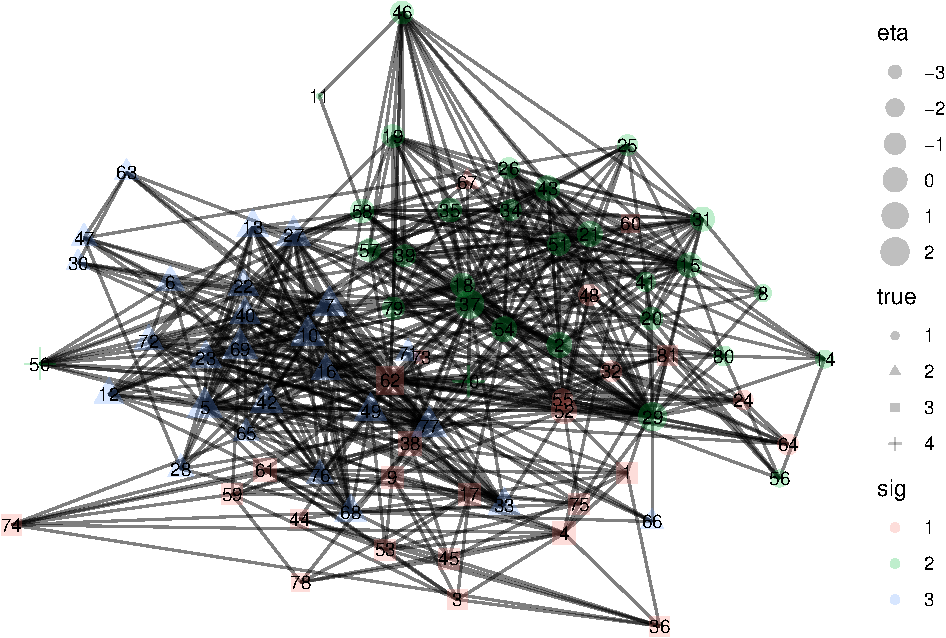
\includegraphics{karate_test_files/figure-latex/unnamed-chunk-19-1.pdf}

\begin{Shaded}
\begin{Highlighting}[]
\KeywordTok{plot_sbmlogit}\NormalTok{(fitK4,}\DataTypeTok{ground =} \StringTok{"school"}\NormalTok{, }\DataTypeTok{alpha =} \FloatTok{0.25}\NormalTok{)}
\end{Highlighting}
\end{Shaded}

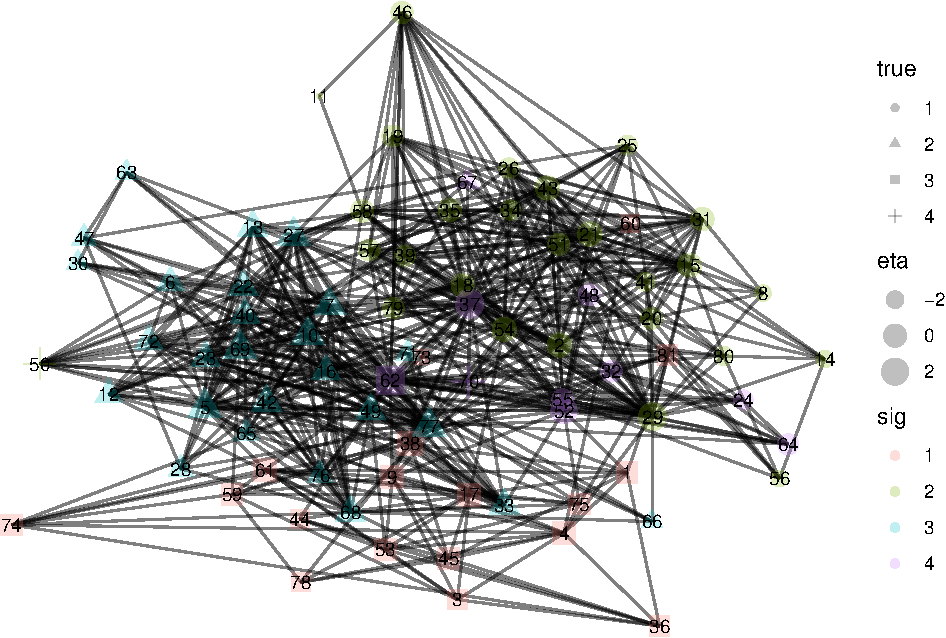
\includegraphics{karate_test_files/figure-latex/unnamed-chunk-20-1.pdf}

\begin{Shaded}
\begin{Highlighting}[]
\KeywordTok{plot_sbmlogit}\NormalTok{(fitK5,}\DataTypeTok{ground =} \StringTok{"school"}\NormalTok{, }\DataTypeTok{alpha =} \FloatTok{0.25}\NormalTok{)}
\end{Highlighting}
\end{Shaded}

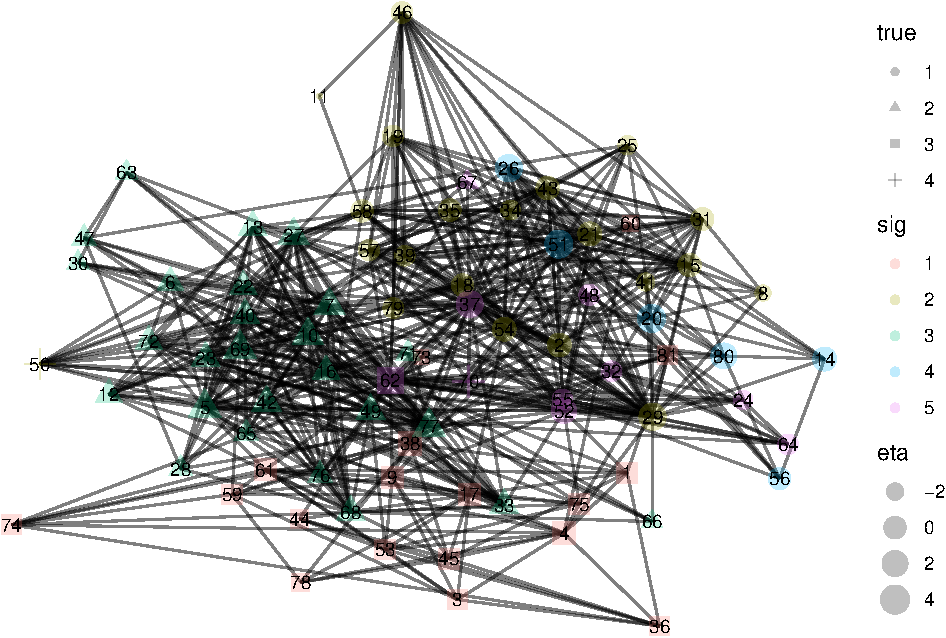
\includegraphics{karate_test_files/figure-latex/unnamed-chunk-21-1.pdf}

For the 4 cluster model, we can assess the degree of community structure
by investigating the \(\gamma\) terms.

\begin{Shaded}
\begin{Highlighting}[]
\KeywordTok{apply}\NormalTok{(fitK4}\OperatorTok{$}\NormalTok{gamma, }\DecValTok{2}\NormalTok{, mean_CRI)}
\end{Highlighting}
\end{Shaded}

\begin{verbatim}
## [1] "-5.68 (-7.21, -4.58)" "-5.15 (-6.4, -4.27)"  "-4.27 (-5.85, -3.26)"
## [4] "-4.54 (-5.25, -3.96)" "-3.08 (-4.24, -2.34)" "-3.68 (-5.01, -2.89)"
\end{verbatim}

It appears there is strong evidence of assortative community structure
in the \texttt{UKfaculty} data since all inter-community \(\gamma\)
parameters are negative and 95\% credible intervals do not contain 0. We
can make sense of the posterior community allotment by relating the
inferred labels to the school membership of each faculty. To do so, we
will obtain the inferred labeling from the \texttt{fitK4} model using
the \texttt{get\_labels()} function, and compare that to the school
membership vector remapped to the canonical space.

\begin{Shaded}
\begin{Highlighting}[]
\NormalTok{sigmaK4 <-}\StringTok{ }\KeywordTok{get_labels}\NormalTok{(fitK4)}
\NormalTok{schools <-}\StringTok{ }\NormalTok{UKfaculty }\OperatorTok
\StringTok{  }\KeywordTok{as_tbl_graph}\NormalTok{() }\OperatorTok
\StringTok{  }\KeywordTok{activate}\NormalTok{(nodes) }\OperatorTok
\StringTok{  }\KeywordTok{pull}\NormalTok{(Group) }\OperatorTok
\StringTok{  }\KeywordTok{sbmlogit.remap}\NormalTok{()}
\end{Highlighting}
\end{Shaded}

\begin{Shaded}
\begin{Highlighting}[]
\KeywordTok{table}\NormalTok{(sigmaK4,schools)}
\end{Highlighting}
\end{Shaded}

\begin{verbatim}
##        schools
## sigmaK4  1  2  3  4
##       1 18  0  0  0
##       2  0 26  0  1
##       3  0  0 26  0
##       4  1  7  1  1
\end{verbatim}

It appears that the inferred communities largely agree with the true
school membership with the exception of the faculty in school 4, of
which there were only 2. The 4 cluster model placed only one of the
faculty from school 4 into cluster 4, but it placed 9 faculty from the
other schools into cluster 4. This suggests that maybe the 3 cluster
model would be a better choice.

\begin{Shaded}
\begin{Highlighting}[]
\NormalTok{sigmaK3 <-}\StringTok{ }\KeywordTok{get_labels}\NormalTok{(fitK3)}
\KeywordTok{table}\NormalTok{(sigmaK3,schools)}
\end{Highlighting}
\end{Shaded}

\begin{verbatim}
##        schools
## sigmaK3  1  2  3  4
##       1 19  6  1  0
##       2  0 27  0  2
##       3  0  0 26  0
\end{verbatim}

From the 3 cluster model, we can see that all faculty from school 1 are
placed in cluster 1, with no other members in cluster 1. The model's
cluster 2 is made up of the 33 members of school 2 as well as the two
members of school 4. The model's cluster 3 is made up of entirely the
faculty of school 3. We can further investigate the parameters of the
three cluster model below.

\begin{Shaded}
\begin{Highlighting}[]
\KeywordTok{apply}\NormalTok{(fitK3}\OperatorTok{$}\NormalTok{gamma, }\DecValTok{2}\NormalTok{, mean_CRI)}
\end{Highlighting}
\end{Shaded}

\begin{verbatim}
## [1] "-3.18 (-4.12, -2.68)" "-3.73 (-5.48, -3.1)"  "-3.82 (-4.42, -3.29)"
\end{verbatim}

From the \(\gamma\) parameters above, we can see that there is strong
assortative community structure in the three cluster model. We can
assess the presence of hub nodes by investigating the \(\eta\)
parameters.

\begin{Shaded}
\begin{Highlighting}[]
\KeywordTok{colMeans}\NormalTok{(fitK3}\OperatorTok{$}\NormalTok{eta) }\OperatorTok\StringTok{ }\KeywordTok{sort}\NormalTok{()}
\end{Highlighting}
\end{Shaded}

\begin{verbatim}
##  [1] -3.422145410 -2.768940997 -1.944328558 -1.850299478 -1.839301326
##  [6] -1.801204060 -1.800914937 -1.688263384 -1.657871911 -1.600569070
## [11] -1.458721109 -1.448636108 -1.221163061 -1.214055872 -1.210175146
## [16] -1.198824474 -1.173434843 -1.051441217 -0.978120244 -0.971834240
## [21] -0.961474131 -0.958884270 -0.948836882 -0.793881229 -0.753810463
## [26] -0.668594399 -0.668510458 -0.643702365 -0.624885202 -0.581931176
## [31] -0.559110886 -0.548181377 -0.533814453 -0.522332856 -0.481830707
## [36] -0.479447664 -0.460727644 -0.456665645 -0.420084814 -0.305991140
## [41] -0.249595939 -0.234259813 -0.155885499 -0.082087696 -0.068478153
## [46] -0.054556791 -0.046120015 -0.025971388 -0.018145317 -0.015207590
## [51] -0.003936638  0.077557049  0.079674630  0.082266014  0.119104636
## [56]  0.216569047  0.367350408  0.388726290  0.388971527  0.400000369
## [61]  0.408638188  0.486256261  0.528342283  0.540110387  0.658911632
## [66]  0.662962871  0.771339578  0.896240426  1.006617277  1.011054726
## [71]  1.081499594  1.125007584  1.201622293  1.436542535  1.450627144
## [76]  1.668261088  1.675715102  1.790963122  2.210299590  2.729701653
## [81]  2.731222360
\end{verbatim}

\begin{Shaded}
\begin{Highlighting}[]
\KeywordTok{geweke.diag}\NormalTok{(fitK3}\OperatorTok{$}\NormalTok{gamma[}\DecValTok{4001}\OperatorTok{:}\DecValTok{5000}\NormalTok{,])}
\end{Highlighting}
\end{Shaded}

\begin{verbatim}
## 
## Fraction in 1st window = 0.1
## Fraction in 2nd window = 0.5 
## 
##   var1   var2   var3 
##  4.328  6.220 -6.188
\end{verbatim}

\end{document}
